\begin{figure}[p]
\centering
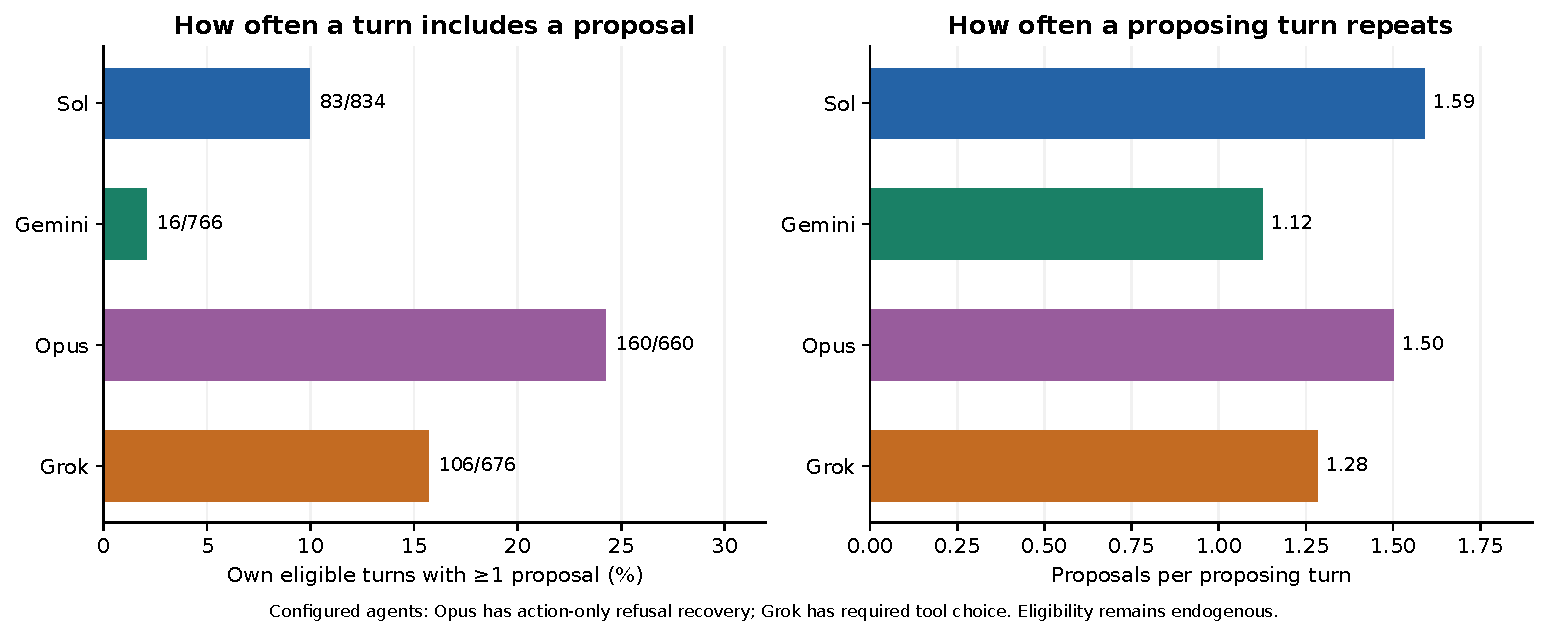
\includegraphics[width=\linewidth,height=4.4in,keepaspectratio]{f03_negotiation_profiles.pdf}
\caption[Negotiation propensity and intensity]{Left: own turns with at least one proposal divided by own turns with an eligible management menu. Right: proposal actions divided by proposing turns. Absolute proposal counts, eligible-decision frequency and decisions per turn remain in the table. Each denominator answers a different question, and survival, access and prior actions affect eligibility. These are activity measures; low initiation does not imply weak recipient bargaining. The table retains all four configured response conditions. Source: Astra's phase-2 negotiation-unit audit.}
\label{fig:f03_negotiation_profiles}
\end{figure}
% Native data cross-reference
\tablenote{Underlying data: Table~\ref{tab:t02_negotiation}.}
